\vspace{-1ex}
\section{Contributions}
%\vspace{-1ex}
\label{sec:contributions}
We have identified the two tasks below as key for translating binaries to compiler IR. We demonstrate the advantages of these two methods through the source-code recovered from a binary corresponding to the example code in Fig~\ref{fig:origCCode}(a).
%shows an example which will be used an an example throughout the following discussion.
%Our techniques for these tasks can be applied to any translation system in general - be it static or dynamic. arguments are 

\noindent $\bullet$ \textbf{Deconstruction of physical stack frames} A source program has an abstract stack representation where the local variables are assumed to be present on the stack but their precise stack layout is not specified. In contrast, a binary program has a fixed (but not explicitly specified) physical stack layout, which is used for allocating local variables as well as for passing the arguments between procedures.
%but where locals and arguments are not listed.The compiler is free to generate any stack layout. 

%(Later in this section, we will create IR symbols for individual stack locations)
To recreate a compiler IR, the physical stack must be deconstructed to individual abstract frames, one per procedure. Since the relative
layout of these frames might change in the rewritten binary, the correct representation requires \emph{all} the arguments (interprocedural accesses through stack pointer) to be recognized and translated to symbols in the IR.
 %layout of these abstract frames might change in the rewritten binary, interprocedural accesses through stack pointer might refer to invalid locations. The correct representation requires \textbf{all} the arguments to be recognized and translated to symbols in the IR.

 %With such an IR, the relative layout of frames might change in the rewritten binary. Consequently, the correctness of physical stack references using the stack pointer from one procedure to a parent or ancestor procedure's frame (common for procedure arguments) no longer holds true. or memory-loaded  This results in undiscovered interprocedural stack accesses, jeopardizing correct recovery of IR. shown (one of many possible) due to the lack of symbolic information

Unfortunately, guaranteeing the static discovery of all the arguments is impossible. Some indirect memory references with run-time-computed addresses might make it impossible for an analysis to statically assign them to a fixed stack location, resulting in undiscovered interprocedural accesses. \emph{Existing frameworks circumvent this problem by preserving the monolithic unmodified stack in the IR, resulting in a low-level IR where no local variables can be added or deleted}.

Some binary analysis tools analyze statically determinable stack accesses to recognize \emph{most} arguments~\cite{gogul04}, aiding limited code understanding. However, the lack of guaranteed discovery of \emph{all} the arguments renders such best-effort techniques insufficient for obtaining a functional IR. Fig~\ref{fig:abstract-stack-diff} shows an example procedure where the first argument \emph{a} can be recognized statically while the second argument \emph{b} is not statically discoverable. In the assembly code, \emph{\&a (esp+20)} is stored to the memory location for \emph{p (esp+8)} (Line 2), which is loaded later to temporary \emph{ecx} (Line 4). The source compiler exploited the layout information (\emph{\&a+4=\&b}) to load \emph{b} by incrementing \emph{p (\&a)} by 4 (Line 5). This is safe since the compiler was able to determine that \emph{p} does not alias \emph{q}. However, the binary framework may not be able to establish this relation, since alias analysis in binaries is less precise. Hence, it has to conservatively assume that the \emph{*q} reference (Line 3) could modify \emph{p} which contained the pointer to \emph{a}. Consequently, the source address at Line 5 is no longer known and argument \emph{b} does not get recognized.

Our analysis in Sec~\ref{sec:deconstructFrame} defines a source-level stack model and checks if the executable conforms to this model. If the model is verified for a procedure, the analysis discovers the arguments statically when possible, but when not possible, embeds run-time checks in IR to maintain the correctness of interprocedural data-flow. Otherwise, stack abstraction is discontinued only in that procedure.
%where a runtime stack is maintained, and stack activation records are created upon procedure entry and destroyed upon exit. of argument data-flow

Fig~\ref{fig:origCCode}(c) demonstrates the impact of abstract stack on the recovered source code. Fig~\ref{fig:origCCode}(b) employs a global pointer \emph{llvm\_ESP}, corresponding to the physical stack frame in the input binary, for interprocedural communication as well as for representing local allocations in each procedure. However, in Fig~\ref{fig:origCCode}(c), the stack pointer disappears; instead, local allocations appear as separate local arrays \emph{llvm\_ESP1} and \emph{llvm\_ESP2} and arguments are passed explicitly.

%Recovering a guaranteed-correct IR gives SecondWrite the advantages of IR listed in section~\ref{sec:intro}, such as unrestricted high-level compiler optimizations and reuse of mature compiler passes. are represented as adjustments of pointer \emph{llvm\_ESP}explicit arguments are  Further, Fig~\ref{fig:origCCode}(c) employs \emph{llvm\_ESP} for interprocedural communication whereas Fig~\ref{fig:origCCode}(b) uses explicit arguments.

\noindent $\bullet$ \textbf{Symbol promotion} Another key challenge we solve is \emph{symbol promotion}, which is the process of safely translating a memory location (or a range of locations) to a symbol in the recovered IR. Existing frameworks do not promote symbols; instead they retain memory locations in their IR~\cite{plto,Diablo1,pintool,dyninst94,newEtch}. Some post-link time optimizers like Ispike~\cite{ispike} promote memory locations to symbols employing the symbol-table information in the object files. However, deployed binaries do not contain symbol information, rendering such solutions unsuitable for our framework.

At first glance, it seems that the well-known methods for variable identification in binaries, such as IDAPro~\cite{ida-pro} and Divine~\cite{reps06}, can be used for symbol promotion. However, this is not the case. The presence of potentially aliasing memory references is a key hindrance to the legal promotion of these identified variables to symbols.
%Variable identification is when binary analysis can discover a variable which is the same as the one defined in the source code. \emph{However, variable identification cannot be used for symbol promotion} because (i) the latter has additional non-aliasing requirements not present in the former; and (ii) symbols recovered need not be the same as the source-code variables. We discuss both below.

IDAPro characterizes statically determinable stack offsets in the program as local variables while Divine divides stack memory region into abstract locations by analyzing indirect memory accesses instructions as well. 
%Divine~\cite{reps06} employs Value Set Analysis (VSA) to aid variable recognition. generating constraints for
%VSA is a combined numeric and pointer analysis which determines an over-approximation of the set of memory addresses as well as the set of integer values that each data object (a register or a memory location) can hold at each program point.  The composition of this stack frame is unknown since the symbolic information is absent in stripped binaries. 

The example in Fig~\ref{fig:ident-prom-diff} illustrates the key limitations of both these methods. When the code is compiled, we obtain a stack frame for \emph{main()} of size 48 bytes (10*4 bytes for array \emph{A[]}, and 4$\times$2 = 8 bytes for the scalars \emph{i} and \emph{x}). The accesses to variables \emph{i} and \emph{x} appear as direct memory references (Lines 3,4,6,9) while the array \emph{A} is accessed using an indirect memory reference (Line 7). Both Divine and IDAPro identify memory locations \emph{(esp+44)(x)} and \emph{(esp+40)(i)} as variables based on the direct references. Since the upper bound for the indirect reference to \emph{A[i]} is statically indeterminable, even Divine does not generate any useful information about this access. Hence, it creates three abstract locations - two scalars of 4 bytes each, and a leftover range of 40 bytes.

\emph{Despite dividing stack memory region into three abstract locations, none of them can be promoted to symbols.} It is impossible to statically prove from the stripped binary that the indirect reference at Line 7 does not alias with references to \emph{i} or \emph{x}. Hence, the promotion of memory locations corresponding to \emph{i} and \emph{x} to symbols would be unsafe since it leads to potentially inconsistent data-flow for underlying memory locations. (Source-level alias analyses often assume that any \emph{A[x]} will access \emph{A[]} within its size. However, such size information is not present in a stripped binary.)
%it is not possible to make this assumption in a binary, since variable size is unknown in absence of symbolic information)
%(Source-level alias analysis methods often assume that A[x] will access A[] within its size, and thus not alias with adjacent variables in the layout. However, it is not possible to make this assumption in the binary, since lacking symbolic information, we do not know what variables are present with what sizes.)

Since identification is inadequate for promotion, we have devised a new algorithm to safely promote a set of memory locations to symbols. It computes a set of non-overlapping promotion lifetimes for each memory location taking into consideration the impact of aliasing memory accesses. Our method is oblivious to the underlying method employed for identifying these locations. The locations can be identified by IDAPro, Divine or through a similar method we use.

Fig~\ref{fig:origCCode}(d) shows the improvement in source code recovery from symbol promotion. Fig~\ref{fig:origCCode}(d) demonstrates the replacement of all access to local array \emph{llvm\_ESP1} and \emph{llvm\_ESP2} in procedures \emph{foo} and \emph{main} respectively by local symbols. As evident, this greatly simplifies the IR and the source code.

%Since identification is inadequate for promotion, we have devised a new promotion method. It identifies possibly aliasing indirect references for each candidate direct reference to be promoted. We divide a procedure into regions, such that there are no aliasing indirect references in that region; hence promotion is safe within the region. To maintain correctness across regions, symbols are loaded from their underlying memory locations upon region entry, and saved upon region exit. In the best case, a region may span an entire function, eliminating the overhead of region-boundary load/stores. Our method to safely promote memory locations to symbols is invariant of the underlying method employed for identifying these locations. The locations can be identified by IDAPro or through Divine.
\noindent {\underline {\textbf{Benefits of abstract stack and symbols}}} The presence of abstract stack and symbols has the following advantages:
\begin{itemize}
\renewcommand{\labelitemi}{\textbf{$\rightarrow$}}
\vspace{-3ex}
\item Improved dataflow analysis since standard dataflow analyses only track symbols and not memory locations.
\item Improved readability of the recovered source-code.
\item The ability to employ source-level transformations without any changes. Advanced transformations like compiler-level parallelization~\cite{ParallelAugust,ParallelSohi} add new local variables as barriers and rely on the recognition of induction variables. Several compile-time security mechanisms like StackGuard~\cite{stackguard} and ProPolice~\cite{propolice1} modify stack layout by placing a \emph{canary} (a memory location) on the stack or by allocating local buffers above other local variables. These methods can be implemented only if the framework supports stack modification and symbol promotion.
\item Efficient reasoning about symbolic memory in case of symbolic execution.
%The inability to perform stack modification and the lack of dataflow analysis of memory locations in existing binary frameworks hinders the direct implementation of such techniques. 
%Further, the absence of enough free registers at the required program points might even make them infeasible. In contrast, we can directly employ the same source-level methods in our rewriter without any changes.between local variables and the return address. Similarly,  changes the stack layout to 
%\item Ability to employ compile-time security defense mechanisms. For example, StackGuard~\cite{stackguard} and ProPolice~\cite{propolice1} modify stack layout by placing a \emph{canary} (a memory location) on the stack or by allocating local buffers above all other local variables. These methods can be implemented only if the framework allows stack modification.

\end{itemize}
 
 %As we explain in Sec~\ref{sec:symExec}, symbol promotion also helps in efficient reasoning about symbolic memory in case of symbolic execution. Further, it improves the applicability of various advanced compiler transformations as explained below.

%The techniques presented in this paper can be applied to any translation system in general - be it static or dynamic. In addition, our method becomes a great platform to statically optimize binaries with future optimizations by other researchers, which may not have been developed yet. We consider this enabling of future methods one of our major contributions, in addition to the run-time improvements in this paper.

%De-constructing the physical stack creates symbols for the stack frame and function arguments. Symbol promotion furthers this process by creating additional symbols within stack frames. The reason symbols help run-time is that dataflow analysis tracks symbols, but not memory locations. Hence every dataflow-based compiler optimization becomes more effective with our symbol-creating methods. This includes standard LLVM optimizations that can be applied to the binary, as well as specialized transformations we have tried, such as automatic parallelization and security enhancement. 
%Examples of how specific advanced optimizations rely on stack modification and symbol promotion are as follows. 

%%\begin{figure}[t]
%\vspace{-0.5in}
%\centering
%\psfig{figure=figures/plots/runtimeFinal.eps,width=5.5in} }
%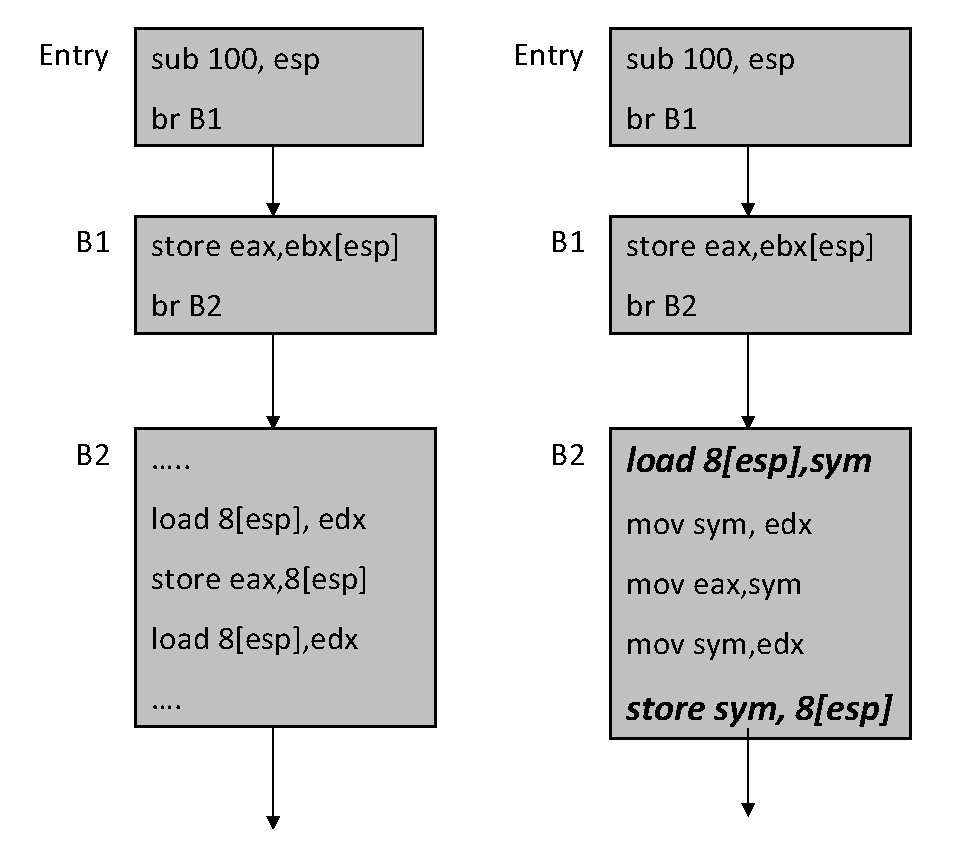
\includegraphics [width=0.5\linewidth] {figures/EPS/cfgex.eps} 
%\tiny{
%\caption { \textit{Stack layout in a binary}}
%}
%\label{fig:stack-layout}
%\end{figure}

\begin{figure}[t]
{
%\begin{minipage}{.5\linewidth}
{
\centering
\includegraphics[width=0.7\linewidth]{figures/EPS/flow1.eps}
\caption{\scriptsize{System Flow}}
\label{fig:systemflow}
\vspace{-0.2in}
}
%\end{minipage}
\hfill
%\begin{minipage}{0.3\linewidth}
%{
%\centering
%\includegraphics[width=\linewidth]{figures/EPS/stackLayout1.eps} 
%\caption{A typical stack layout}
%\label{fig:stacklayout}
%}
%\end{minipage}
\vspace{-0.2in}
}
\end{figure}

Fig~\ref{fig:systemflow} presents an overview of our framework. SecondWrite produces an initial LLVM IR using custom binary reader modules. The initial IR is enhanced using the above mentioned techniques to obtain an enhanced IR, which can be employed for multiple applications described in Sec~\ref{sec:intro}.

%The frontend module in \emph{SecondWrite} system, consisting of a disassembler and a custom reader module, processes the individual instructions in input executable and generates an initial LLVM IR. This initial representation is devoid of the desired IR features like abstract stack frame and symbols. This initial IR is analyzed to obtain an improved IR which has all the information and features mentioned previously. The standard suite of LLVM optimizations and various new optimization passes can be applied on the above IR to get an optimized IR. The optimized IR is finally passed to the existing LLVM code generator to obtain the rewritten binary. The C backend present in LLVM compiler can be used to obtain C code for better analysis of executables.
%\footnote{Indirect calls and branches occurring in the original binary are handled by translating their target addresses in relocation tables when present in the binary, or through a custom binary rewriting technique we are developing when such tables are absent. However, the choice of technique is orthogonal to the techniques presented in this paper and does not affect our analysis}. 

%Symbol promotion also helps in efficient reasoning about symbolic memory in case of symbolic execution. The symbolic memory address problem arises whenever an address referenced in a load or store operation is an expression derived from user input. Various existing symbolic execution systems either make unsound assumptions by concretizing the symbolic addresses to a fixed value or employ SMT solvers to reason about possible locations accessed. 

%Apart from making dataflow analyses more effective, the promotion of memory locations to symbols improves the efficiency of various backend optimizations like register allocation. It enables the register allocator present in a binary rewriter to undo the decisions made by the original compiler and enables it to take full advantage of any additional registers present in the target end-user platform (e.g more \emph{xmm} and general purpose registers on X86-64).
%For example, the techniques presented by Li et al~\cite{dyn-reg-prom11} for dynamically promoting variables to additional registers in the target architecture would substantially benefit from our techniques due to the availability of more symbols.

%In summary, following are the main contribution of this work:\\
%	- A novel binary rewriting framework based on a compiler intermediate representation \\
%	- Methods for deconstruction of physical stack frames in binary to abstract stack frames.\\
%	- A partition based algorithm for symbol promotion of memory locations.

\vspace{-.4ex}
